%!TEX root = ../dissertation.tex

	
\newcommand{\ind}{\perp \!\!\! \perp}
\newcommand{\exposure}[1]{\textrm{Exposure}(#1|\mathbf{P})}

\chapter{Background on Fairness in Rankings}\label{chapt:background}


As discussed in the Introduction, the goal of algorithmic fairness is to make sure that the decision-making algorithm does not discriminate against protected subgroups of the population. But that is a rather nebulous definition: what do we mean by «discriminate»? How do we tell if an algorithm is «fair» or not?

In section 2.1, I will attempt to answer these questions with arguments based mainly the work of Friedler et al. \cite{1609.07236} and Zehlike et al. \cite{3533379}, \cite{3533380}. Then, in section 2.2, I will describe and contrast the two approaches that divide the field of FairML: Individual vs. Group Fairness. Finally, in section 2.3, I will lay out the mathematical formulation of some metrics used to quantify fairness in ranking.

\section{Worldviews}\label{sect:1_1}

As we shall see in the next section of this chapter, there are many quantitative measures of algorithmic fairness. However, \cite{1609.07236} notes that they are oftentimes introduced «ad-hoc», without stating the assumptions underlying them. The authors introduce the idea of three spaces, such that any measure of fairness may be classified according to the assumptions it makes about interactions between them.

Those are the Construct space (CS), the Observed space (OS) and the Decision space (DS). A representation of them is shown on Fig. X. The Construct space  represents the true properties of an individual in which the decision-maker is interested –e.g., their intelligence. However, those properties are unobservable directly – in the real world, we have to rely on proxies, like, for example, test scores; those lie in the Observed space. The Decision space is made up of the decisions made by the model – binary «yes/no» in case of classification, a number in case of regression, and the individual’s position in case of ranking.

\begin{figure}[t]
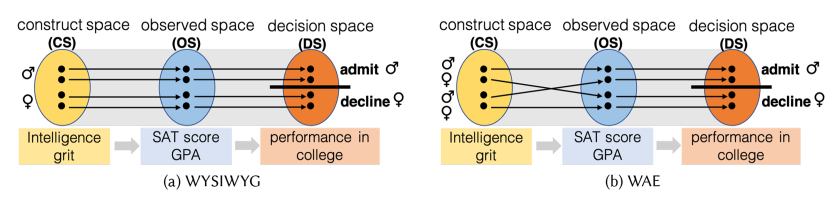
\includegraphics[scale=0.8]{resources/worldviews.png}
\centering
\caption{An illustration of worldviews from Frieder et al. \cite{1609.07236}. WYSIWYG worldview assumes minimal disortion between the construct space (CS), that contains actual quantites of interest - e.g. intelligence and the observed space (OS), that contains observations - e.g. test scores. WAE worldview assumes that the mapping from the CS and OS treats different groups differently to a non-negligible degree - e.g. women's test scores being artificially lowered compared to men's.}
\label{fig:ch1_worldviews}
\end{figure}

As the paper notes, any fairness metric implies assumptions about how those spaces interact. Those can be divided into two worldviews: «What You See Is What You Get» (WYSIWYG) and «We are All Equal» (WAE).

\textbf{WYSIWYG} denotes the belief that the differences between the OS and the CS are minimal, thus it is possible to accurately compare each candidate’s true quantity of interest (e.g. a university applicant’s ability) using just the observations (their exam scores).

\textbf{WAE} worldview, on the other hand, assumes that in the CS, all groups look essentially the same – all qualities relevant to the decision-making process are distributed nearly identically within each group. The reason WAE gives for observed differences is that the transformation from the CS to the OS is inaccurate and treats different groups in different ways. In this worldview, OS is an unreliable representation of the CS: for example, a physics exam taken in English may be representative of the physics knowledge of an English-speaking student, but not of a non-English-speaking one.

When designing a fairness-oriented algorithm, it is necessary to choose between the two worldviews. In some ways, they correspond to different concerns a model designer might have: roughly speaking, WYSIWYG means that we trust the data to provide an accurate representation of the CS, and are concerned with the model itself learning to discriminate on the unwanted attributes from data; while WAE means that we think the data is biased due to real-world issues and want the model to correct for that.

While the question of worldviews may seem purely theoretical, it is necessary for a deeper understanding of a much more practical choice in the field of Fair ML: Individual versus Group fairness.


\section{Individual vs. Group Fairness}\label{sect:1_2}

The first definition to arise in the field of Fair ML was \textbf{group fairness}. Group fairness is simple: it asks for the model output to be independent of group membership; given the model output $R$ and group membership $A$, it requires that 
\[
P(R=1|A=a) = P(R=1|A=b)
\]

It is also known as demographic parity, statistical parity, or disparate impact. Under the last name, and with a relaxed formulation, it is widely employed in legal settings - take, for example, the “four-fifths” rule in the USA that requires the job acceptance rate for each significant protected group to be at least 4/5 of that of the most frequently accepted group.

\textbf{Individual fairness}, on the other hand, aims for similar individuals to be treated similarly. It was introduced into the field of Fair ML in \cite{dwork2011fairness}; there, the similarity between individuals is measured with a user-defined metric. The authors recognize that designing a «fair» metric is a difficult problem, as there might be structural bias present in the data.

A widespread set of fairness criteria that aims for individual fairness is equalized odds and equality of opportunity, which require, respectively, equal error rates and equal false positive rates across groups. They are based on either full or relaxed statistical notion of separation: the output $R$ is separated from the group membership A by the ground truth Y if $R \ind A | Y$. It makes intuitive sense in a classification setting if we consider Y as a measure of merit: equally qualified individuals should be accepted or refused with equal rates, regardless of their group membership.

It is easy to see how the individual and group fairness notions map closely to the WYSIWYG vs. WAE worldviews, respectively. More accurately, as pointed out in \cite{1609.07236}, individual fairness requires the user to assume the WYSIWYG worldview to guarantee fairness, and vice versa (note that, unlike the paper, in this thesis I do not make a distinction between “fairness” and “non-discrimination”, because this section is intended only to provide a basic theoretical background).

There are apparent tradeoffs to choosing between individual and group fairness, which have roots in the conflict between WYSIWYG and WAE. Using our running example, if we assume that the students’ test scores accurately represent their intelligence (WYSIWYG), adhering to individual fairness criteria would make sure that students with similar scores would have the same probability of acceptance, regardless of race; on the other hand, if we know the tests to favor one group over the others (WAE), individual fairness would just reinforce that difference.

Similarly, the disadvantages of group fairness under WYSIWYG are apparent: by forcing the model to produce similar outputs regardless of group membership, it would unfairly «elevate» black students with lower scores. Group fairness constraints can even be used insidiously: a recruiter may hire candidates from the privileged and protected groups at the same rate, but purposefully select less qualified members of the latter; this would lead to worse performance from the protected group, which can be used to justify further discrimination \cite{fairmlbook}. In the real world, this is known as the «glass cliff» phenomenon.


\section{Measuring Fairness in Rankings}\label{sect:1_3}

Having established the theoretical basis behind different fairness criteria, we can finally move on to their mathematical formulation. As stated already, most work on fairness focuses on the problem of classification, and thus, a wide range of metrics has been introduced for this task, focusing on both group (positive classification rate) and individual (false positive rate ratio, false negative rate ratio, error rate ratio, and so on) fairness \cite{1810.08810}.

Much less work has been put into the problem of rankings, however. Biega et al. \cite{equityofattentionBiega} choose the individual approach (WYSIWYG) and aim to ensure that the user attention received by each item is proportional to the item’s relevance to a given query. As a proxy for attention, they use position-based discounts – a quantity that decreases as the item is placed further down in the ranking, e.g. $p(1 - p)^{(j-1)}$ for a user-set parameter $p$ and position $j$. The authors argue that their constraints are unlikely to be achieved in any single ranking, so they attempt to optimize cumulative attention received by items over multiple successive rankings (e.g. multiple repeated responses to the same internet search query, or even to different queries – in which case the items’ relevance scores will change depending on the query):

$$
  \frac{\sum_{l=1}^{m} a^l_{i1}}{\sum_{l=1}^{m} r^l_{i1}} 
= \frac{\sum_{l=1}^{m} a^l_{i2}} {\sum_{l=1}^{m} r^l_{i2}},\ \forall u_{i1}, u_{i2}.
$$,
where $u_{i1}, u_{i2}$ are a pair users, $a^l_{i1}, a^l_{i2}$ are the normalized attention values received by the two users in ranking $l$, and $r^l_{i1}, r^l_{i2}$ are the normalized relevance values of the two users in the ranking $l$.

In \cite{FairnessofExposureSJ}, the authors introduce constraints for both individual and group fairness based on the notion of exposure:

\[
\exposure{d_i} = \sum_{j=1}^N \mathbf{P}_{i,j} v_j
\]


Where $X_a$ is the item, $P_{a,i}^{\tau}$ is the probability of the model placing the candidate $a$ at rank $i$ in ranking $\tau$, and $v(i)$ is the position discount.

The average exposure of a group $G_k$ is defined as:

\[
\exposure{G_k}=\frac{1}{|G_k|}\sum_{d_i \in G_k} \exposure{d_i},
\]

In the individual case (WYSIWYG), the aim is to guarantee that the average exposure of each group is proportional to the average utility of its items; in the group case (WAE), the average exposure is required to be equal across all groups.

Finally, \cite{fair}, \cite{linkedin} and \cite{RAPF} place firm constraints on the group structure of the rankings. These works aim to achieve equal representation of groups in the top k entries – also known as proportional, or proportionate, fairness.

For each position $i$ and protected group $g$, \cite{fair} introduces a lower bound $\alpha_i$ such that the proportion of members of protected groups does not fall too far below a user-set percentage $p$. As the main contribution of the paper is an algorithm that constructs a sub-ranking of size $k$ out of a larger set of scored candidates, the fairness of the result is evaluated using the percent of protected candidates in the sub-ranking. While this approach is intuitive, it does not account for the positions of the candidates: for example, all individuals belonging from the protected group may be situated at the bottom.

\cite{linkedin} introduced the InfeasibleIndex metric, defined as the number of positions at which the lower representation bound is violated:

\begin{equation}
\label{eq:infeasible_index}
\textrm{InfeasibleIndex}(\pi) = \sum_{k=1}^{|\pi|} 1{(\exists G_i \in G, ~s.t. ~ \text{count}_k(G_i, \pi) < \lfloor \alpha_i \cdot k \rfloor)}.
\end{equation}

where $\tau_r$ is the ranking, $G$ is the set of groups, $\alpha_i$ is the lower constraint on the proportion of items of group $G_i$ in the ranking set by the user.

\cite{RAPF} improved on that by also considering the upper bound in the “Percentage of P-Fair Positions” – or the percentage of positions in the ranking at which none of the requirements are violated. The authors claim that introducing an upper representation constraint in addition to the lower one provides for more robust fairness guarantees.

In this work, I use the latter metric, as well as a modification of InfeasibleIndex that also counts the upper bound violations:

%\begin{equation}
\begin{align*}
    \text{LowerViol}(\pi) & = \sum_{k=1}^{|\pi|} 1{(\exists G_i \in G, ~s.t. ~ \text{count}_k(G_i, \pi) < \lfloor \alpha_i \cdot k\rfloor} \\
%
\text{UpperViol}(\pi) &= \sum_{k =1}^{|\pi|} 1{(\exists G_i \in G, ~s.t. ~ \text{count}_k(G_i, \pi) > \lceil \beta_i \cdot k\rceil}\,
\end{align*}
%
where $\text{count}_k(G_i, \pi)$ is the number of elements of group $G_i$ in the top $k$ positions of ranking $\pi$; $\alpha_i, \beta_i$ are the lower and upper constraints on the proportion of items of that group in the ranking. Then,  %
\[
\text{TwoSidedInfInd}(\pi) = \text{LowerViol}(\pi) + \text{UpperViol}(\pi) 
\]
%\end{equation}

Depending on the choice of the proportions for each group, these metrics can describe both individual and group fairness, as noted in \cite{linkedin} and \cite{RAPF}. In this thesis, the focus will be placed on group fairness.







